%UNIT 3: RATIONAL NUMBER OPERATIONS - WORKSHEET 2
\documentclass[12pt, letterpaper, fleqn]{article}

% ----------------------------------------------------------
% PACKAGES
% ----------------------------------------------------------
\usepackage{graphicx}
\usepackage{xcolor}
\usepackage[most]{tcolorbox}
\usepackage{amsmath, amssymb}
\usepackage{fancyhdr}
\usepackage[utf8]{inputenc}
\usepackage[T1]{fontenc}
\usepackage{enumitem}
\usepackage{geometry}
\usepackage{tikz}
\usepackage{needspace}
\usepackage{multicol}

\usetikzlibrary{arrows.meta, calc}

% ----------------------------------------------------------
% PAGE SETUP
% ----------------------------------------------------------
\usepackage{times}
\geometry{letterpaper, top=1.25in, bottom=1.25in, marginpar=0.5in}

% ----------------------------------------------------------
% HEADER / FOOTER
% ----------------------------------------------------------
\newcommand{\logowidth}{3cm}
\setlength{\headheight}{20pt}
\setlength{\footskip}{40pt}

\pagestyle{fancy}
\fancyhf{}
\fancyhead[C]{\small\bfseries Adding & Subtracting Rational Numbers}
\fancyfoot[L]{\raisebox{2pt}{
\includegraphics[width=\logowidth]{kss.png}}}
\fancyfoot[C]{\thepage}
\fancyfoot[R]{7.6.2}

\renewcommand{\footrulewidth}{0.2pt}

% ----------------------------------------------------------
% THEME COLOR
% ----------------------------------------------------------
\definecolor{customteal}{HTML}{2fbdb9}

% ----------------------------------------------------------
% HELPER MACROS
% ----------------------------------------------------------
\newcommand{\blank}{\underline{\hspace{2.2cm}}}
\newcommand{\blanklong}{\underline{\hspace{6.5cm}}}
\newcommand{\blankshorter}{\underline{\hspace{1.5cm}}}

% ----------------------------------------------------------
% DOCUMENT
% ----------------------------------------------------------
\begin{document}

\textbf{Name:} \underline{\hspace{5cm}}
\hfill
\textbf{Date:} \underline{\hspace{3cm}}\\

% ==========================================================
% PART A — NUMBER LINES & COMPUTATION
% ==========================================================
% --- PART A ---
\begin{tcolorbox}[colback=customteal!20]
\large\textcolor{black}{\textbf{Part A: Number Line Representations \& Computation}}
\end{tcolorbox}

\vspace{3mm}

\begin{enumerate}[itemsep=4.2cm, leftmargin=0.6cm]
\item Examine the number line model below. Write the addition equation (using rational numbers) represented by the arrows, and find the final sum.

\begin{center}
\begin{tikzpicture}[x=1.1cm, y=0.8cm]
    % Draw number line
    \draw[latex-latex, thick] (-4.5,0) -- (4.5,0);
    \foreach \x in {-4,-3,-2,-1,0,1,2,3,4}
        \draw (\x,0.15) -- (\x,-0.15) node[below] {\small \x};
    
    % First vector (0 to -1.5)
    \draw[thick, -latex, blue] (0,0.5) -- (-1.5,0.5);
    \node[above, blue] at (-0.75,0.5) {\small $-1.5$};
    
    % Second vector (-1.5 to 2.5)
    \draw[thick, -latex, red] (-1.5,1.1) -- (2.5,1.1);
    \node[above, red] at (0.5,1.1) {\small $+4.0$};
\end{tikzpicture}
\end{center}

\textbf{Equation:} \blanklong
\item Use the blank number line below to model the expression: \textbf{$-2 + \left(-1\dfrac{1}{2}\right)$}. Draw the arrows and state the final value.

\begin{center}
\begin{tikzpicture}[x=1.1cm, y=0.8cm]
    % Draw blank number line
    \draw[latex-latex, thick] (-5.5,0) -- (1.5,0);
    \foreach \x in {-5,-4,-3,-2,-1,0,1}
        \draw (\x,0.15) -- (\x,-0.15) node[below] {\small \x};
\end{tikzpicture}
\end{center}

\textbf{Value:} \blank
\end{enumerate}

\newpage

% --- PART B ---
\begin{tcolorbox}[colback=customteal!20]
\large\textcolor{black}{\textbf{Part B: Number Line Representations \& Computation}}
\end{tcolorbox}

\vspace{3mm}

\begin{enumerate}[itemsep=4.2cm, leftmargin=0.6cm, resume]
\item Find the sum or difference. Show your steps clearly.
\begin{enumerate}[label=\alph*., itemsep=\fill]
\item $-5.8 + (-3.4) =$ \blank
\end{enumerate}

\newpage

% --- PART C ---
\begin{tcolorbox}[colback=customteal!20]
\large\textcolor{black}{\textbf{Part C: Number Line Representations \& Computation}}
\end{tcolorbox}

\vspace{3mm}

\begin{enumerate}[itemsep=4.2cm, leftmargin=0.6cm, resume]
\item $-\dfrac{5}{6} - \left(-\dfrac{1}{3}\right) =$ \blank
\item $4\dfrac{1}{4} - 6\dfrac{1}{2} =$ \blank
\end{enumerate}

\newpage

% --- PART D ---
\begin{tcolorbox}[colback=customteal!20]
\large\textcolor{black}{\textbf{Part D: Number Line Representations \& Computation}}
\end{tcolorbox}

\vspace{3mm}

\begin{enumerate}[itemsep=4.2cm, leftmargin=0.6cm, resume]
\item \textbf{Temperature Change:} At 5:00 AM, the temperature in Minneapolis was $-8.5^\circ\text{F}$. By noon, the temperature had risen by $15.3^\circ\text{F}$. What was the temperature at noon?
\\
\textbf{Expression:} \blanklong \\
\textbf{Answer:} \blanklong
\item \textbf{Elevation:} A research submarine is cruising at an elevation of $-120.5$ meters (relative to sea level). It then descends another $45\dfrac{1}{4}$ meters to collect soil samples. What is the submarine's new elevation?
\\
\textbf{Expression:} \blanklong \\
\textbf{Answer:} \blanklong
\item \textbf{Personal Finance:} Marcus has a balance of $-\$22.50$ in his checking account. He deposits a birthday check for $\$50.00$, and then uses his debit card to buy a book for $\$12.75$. What is Marcus's new account balance?
\\
\textbf{Expression:} \blanklong \\
\textbf{Answer:} \blanklong
\item \textbf{Distance on a Number Line:} Find the distance between $-3\dfrac{1}{2}$ and $2.75$ on a horizontal number line. Explain how you can use absolute value to find this distance.
\item \textbf{Analyzing Error:} Clara tried to solve the expression $-4.5 - (-2.1)$. Her work is shown below:
\begin{align*}
    &-4.5 - (-2.1) \\
    &= -4.5 - 2.1 \\
    &= -6.6
\end{align*}
Identify Clara's error, explain what she did wrong, and provide the correct solution.
\end{enumerate}

\end{document}
